\section{Task Description}

% Find additional features in primary/secondary care (PSC) databases and from spatial analyses
The analyses presented so far have used variables in, or derived from, the ACE referral form. Consequently, these variables represent data that the ACE admissions team have access to at the point of deciding whether to accept a referral. Considering this, it may therefore be unsurprising that predictive models trained on that data are not able to outperform experienced healthcare professionals.

The aim of this chapter is to investigate additional sources of data beyond the ACE referral form. By linking this data to that derived from the ACE referral form, we intend to build a model that may have increased predictive power over those built just using ACE data. We also aim to flag any variables of high predictive power that may be useful for the ACE team to consider as part of their acceptance criteria.

\section{Experimental set-up}

\subsection{Data sources}
\label{sec:additional-data-sources}

The additional features used throughout this chapter fall into two main groups: Those derived from primary and secondary care (PSC) records, and those derived from geographical and geospatial analyses. 
% PSC from CY
PSC data were obtained from Connected Bradford (cBradford), an anonymised database linking routine electronic health data across primary, secondary, social and community care for over 700,000 individuals across Bradford Teaching Hospitals NHS Foundation Trust.

% Air & IMD
The geospatial analyses fell into three categories: Air quality measures, indices of multiple deprivation (IMD) and distance measures. Estimated background air pollution maps based on 2018 were downloaded from the DEFRA website (\href{https://uk-air.defra.gov.uk/data/laqm-background-home}{found here}). IMD data from 2019 were downloaded from the Ministry of Housing, Communities and Local Government's GIS team (\href{https://data-communities.opendata.arcgis.com/datasets/5e1c399d787e48c0902e5fe4fc1ccfe3/about}{found here}). Co-ordinates of GP surgeries and hospitals in the Bradford area were obtained using Google Maps.

\subsection{Features from ACE referral form}

The following features derived from the ACE referral form were included in the modelling process: Age, gender, illness severity, activity level, oxygen saturation, respiratory rate, heart rate, temperature, safeguarding concerns, food allergies, drug allergies, other allergies, whether the patient met the ACE referral criteria, mention of `asthma' in the medical history, mention of `salbutamol' in the examination notes, whether the referral was made by the GP, respiratory rate outside of the `normal' APLS category, heart rate outside of the `normal' APLS category, and whether the examiner's `gut feeling' was anything other than `normal'. Specific definitions of these variables can be found in the previous sections of this report.

\subsection{Variables of interest}

After data extraction and variable definition (detailed below in \Cref{sec:PSC-features} and \Cref{sec:geospatial-features}), variables were tested in univariate binary logistic regression models with hospitalisation as the response variable. Those showing a both significant (\textit{p}<0.05) association with hospitalisation, and occurrence in at least 5\% of the total patient population were termed `variables of interest'. In total, 37 `variables of interest' beyond the variables extracted from the ACE referral form were identified and carried forward to further analysis.

\subsection{Primary/secondary care features}
\label{sec:PSC-features}

% Extraction process and definitions
Raw data were extracted from cBradford using SQL scripts built on a subset of the database (containing ~5\% of the total patients), then run on the main database. Four main categories of data were extracted, and are detailed below. 

\subsubsection{Demographics}

% Variables extracted
Gender and ethnicity were extracted from cBradford, although these variables also already existed in the ACE referral form. Ethnicity was grouped into `Pakistani', `White' and `Other'. 
% Variables of interest -> None!
Neither of these variables influenced hospitalisation risk (see \Cref{tab:additional-demographics-table}), and thus none were carried forward to modelling.

\subsubsection{Co-morbidities}

% Variables extracted
As this work uses data from the `asthma/wheezy child' ACE pathway, we extracted information on a number of conditions known to be co-morbid with asthma \cite{Boulet2009}. Full details of co-morbidity data extracted are shown in \Cref{tab:additional-comorbidity-table}. From co-morbidity occurrence dates, binary variables were created for each condition determining whether diagnosis occurred within the month, six months, or year before ACE acceptance, as well as whether a diagnosis of the condition had ever been made.

% Variables of interest
Co-morbidity `variables of interest' were any diagnoses of eczema, pneumonia, bronchitis, and of any other `common respiratory conditions' (Influenza, common cold, hay fever, sinusitis, croup and streptococcal pharyngitis), as well as diagnosis of eczema in the last year (before ACE acceptance), pneumonia in the last year, and eczema in the last six months. Further details on these variables are found in \Cref{tab:additional-comorbidity-interest}. 

\subsubsection{Prescriptions}
% 

Data were extracted on the prescription (and frequency) of four main categories of medication: Fast-acting bronchodilators (\textit{relievers}), slow-acting bronchodilators (\textit{preventers}), antihistamines, and prednisolone (see \Cref{tab:additional-prescription-table}). Data were also extracted on the number of inhalers prescribed prior to ACE acceptance.

As with co-morbidity data, prescription data were used to construct binary variables measuring if (and if so, how many times) prescription occurred during the year, six months and month prior to acceptance. Variables of interest (\Cref{tab:additional-prescriptions-interest}) were the prescription of slow bronchodilators at all, within the last year, and within the last month, and the prescription of prednisolone within the last year, and within the last six months.

% Binarised variables
Also of interest were several binarised variables (see \Cref{sec-additional-binarisation}): \textgreater 12 total inhalers prescribed before ACE acceptance, >4 total courses of prednisolone, >3 courses of prednisolone in the last year, and >4 courses of prednisolone in the six months.

\subsubsection{Visits}
% 
Data were extracted on the number of visits to different healthcare facilities made by patients prior to ACE admission. These were the emergency room (ER), general practice (GP), a hospital as an outpatient (OP), and a hospital as an inpatient (IP) (\Cref{tab:additional-visit-table}). The number of visits within 3 years, one year, six months and one month of ACE acceptance were totalled.

Binarised variables of interest (\Cref{tab:additional-visits-interest}) consisted of >4 visits to the ER in the last year, >6 visits to the GP in the last year, >4 visits to the GP in the last six months, >9 IP visits in total,  >4 IP visits in the last 3 years, >2 IP visits in the last year, >1 IP visit in the last 6 months, >8 visits of any kind in the last year, >4 visits of any kind in the last six months, and >6 visits of any kind in the last month.

\subsection{Geospatial features}
\label{sec:geospatial-features}

The geospatial measures were calculated at the Lower Layer Super Output Area (LSOA) level, as this is the finest spatial scale to which patient data was available. Each LSOA is of comparable population, with a minimum of 1,000 people and a mean of 1,500. As the full ACE dataset contained patients from 172 unique LSOAs, LSOA could not be included in any model as its own covariate. Moreover, increased hospitalisation associated with certain specific LSOAs would give little information on \textit{why} those patients were at higher risk of hospitalisation. Thus, we calculated three main families of continuous geospatial features which allowed analysis of the factors influencing any geographic variation in hospitalisation risk.

\subsubsection{Air quality measures}

% How measured
The three main metrics of air quality used were nitrogen dioxide (NO$_2$), particles < 10$\mu$m (PM$_{10}$), and particles < 2.5$\mu$m (PM$_{2.5}$). These metrics were in the form of estimated mean concentrations (in $\mu$g$\cdot$m$^3$) obtained from DEFRA background data (see \Cref{sec:additional-data-sources}) on a 1$\times$1 km$^2$ grid. 
% Measured postcodes within LSOA
For each postcode within an LSOA, we measured the nearest air quality estimate, then took the value for the LSOA to be the mean of all postcodes within the LSOA.

Summaries of the three measures are shown in \Cref{tab:additional-air-table}. Whilst none of the three measures showed a linear relationship with hospitalisation risk, NO$_2$ and PM$_{10}$ counted as `variables of interest' after binarisation (\Cref{tab:additional-air-interest}). As such, NO$_2$ > 18.75 $\mu$g$\cdot$m$^3$ and PM$_{10}$ > 13.5 $\mu$g$\cdot$m$^3$ were carried forward to modelling.

\subsubsection{Indices of Multiple Deprivation}

% Already on LSOA level - 16
The data on indices of multiple deprivation were already provided at the LSOA level. They comprised 16 variables in total: 9 scores and 6 sub-domain scores, which are combined to calculate the total IMD score. The 9 main scores are: `Barriers to housing and services', `Crime', `Education, skills and training', `Employment', `Living environment', `Health deprivation and disability', `Income deprivation affecting children', `Income deprivation affecting older people', and `Income'. The 6 sub-domain scores are: `Adult skills', `Children and young people', `Geographical barriers', `Indoors', `Outdoors' and `Wider barriers' (\Cref{tab:additional-IMD-table}).

Whilst these scores are also available as deciles, we kept them as continuous numerical scores in order to conserve model degrees of freedom. None of the scores showed a linear relationship with hospitalisation risk, but three showed a relationship following binarisation - `Children and young people' sub-domain score, `Education, skills and training' score and `Income deprivation affecting children' score (\Cref{tab:additional-IMD-interest}).

\subsubsection{Distance measures}

% Measured euclidian from centroid
From the centroid of each LSOA, we measured the distance to each GP surgery, as well as the distance to the closest hospital (either St Luke's or the Bradford Royal Infirmary). We measured simply Euclidean distance; as we were measuring from LSOA centroids, rather than patient's postcodes or houses directly, there was little advantage to be gained from measuring actual travel distances or times.

The log-transformed distance from the LSOA in which a patient lived to their GP surgery showed a significant relationship with hospitalisation risk, and was thus included as a variable of interest (\Cref{tab:additional-distance-table}). After binarisation, both standard and log-transformed distances to GP surgeries and to the nearest hospital were all included as variables of interest (\Cref{tab:additional-distance-interest}).

\subsection{Binarisation of continuous variables}
\label{sec-additional-binarisation}

To allow for potential non-linearities in the relationship between continuous variables and hospitalisations, we performed an automated binarisation process to yield a split point, above which the variable would be classed as `high', and below which it would be low. The best binarisation threshold for each variable was found by iterating the following process:

\begin{enumerate}
\item Select a candidate binarisation threshold.
\item Binarise the variable and fit a logistic regression model with the binary variable as the explanatory variable, and hospitalisation as the response variable.
\item Calculate a 95\% confidence interval on the resulting coefficient
\item Record the difference between the upper and lower confidence limits, and whether the confidence interval overlaps with zero 
\end{enumerate}

The above process was followed for all possible binarisation thresholds. The best threshold was taken as the one that produces the narrowest confidence interval (i.e., smallest difference between lower and upper limit) where the limit does not include zero. If all tested confidence intervals overlapped with zero, the variable was not carried forward to modelling. Binarisation thresholds for all variables of interest are shown in the tables in \Cref{sec:app-additional-features}.

\subsection{Outcome measure}

% Hosp in subset that are on CY
As with previous chapters, our outcome measure is whether hospitalisation was required following acceptance onto the ACE service. Unlike in previous chapters, however, not all data from the ACE referral form dataset can be used, as only a subset of these patients (n = 446) had data on cBradford available for linkage. Of these, n = 78 (17.4\%) were admitted to hospital.

\subsection{Determining model structure}
\label{sec:additional-model-structure}

Two datasets, and thus two models, were created and assessed. The first, termed `Original' comprised only variables extracted or engineered from the ACE referral form. The second, termed `Additional', also contained the additional features detailed above.

% Lasso
The variables retained in each models (and thus, the structure of each model) was determined by least absolute shrinkage and selection operator (lasso) logistic regression, with hospitalisation as the response variable, and all other variables as explanatory variables. Lasso regression works by a shrinkage parameter $\lambda$ which penalises very small coefficient estimates, setting them to zero; the greater the value of $\lambda$, the fewer non-zero coefficients remain in the final model \cite{Tibshirani2011}.

% Finding lambda
We profiled a range of potential $\lambda$ values and selected a final value which yielded a model with the best adherence to the `10 events per variable' rule-of-thumb \cite{Austin2017}. This rule suggests that for a binary outcome, a prediction model should have one additional degree of freedom per 10 positive cases. With a total of 78 positive cases, this allows for a model with 8 degrees of freedom (equating to 8 variables, since all variables in both datasets are either binary or continuous, adding only one degree of freedom).

\subsection{Bootstrap aggregation modelling}

% Flowchart and overview
\begin{figure}[h]
    \centering
    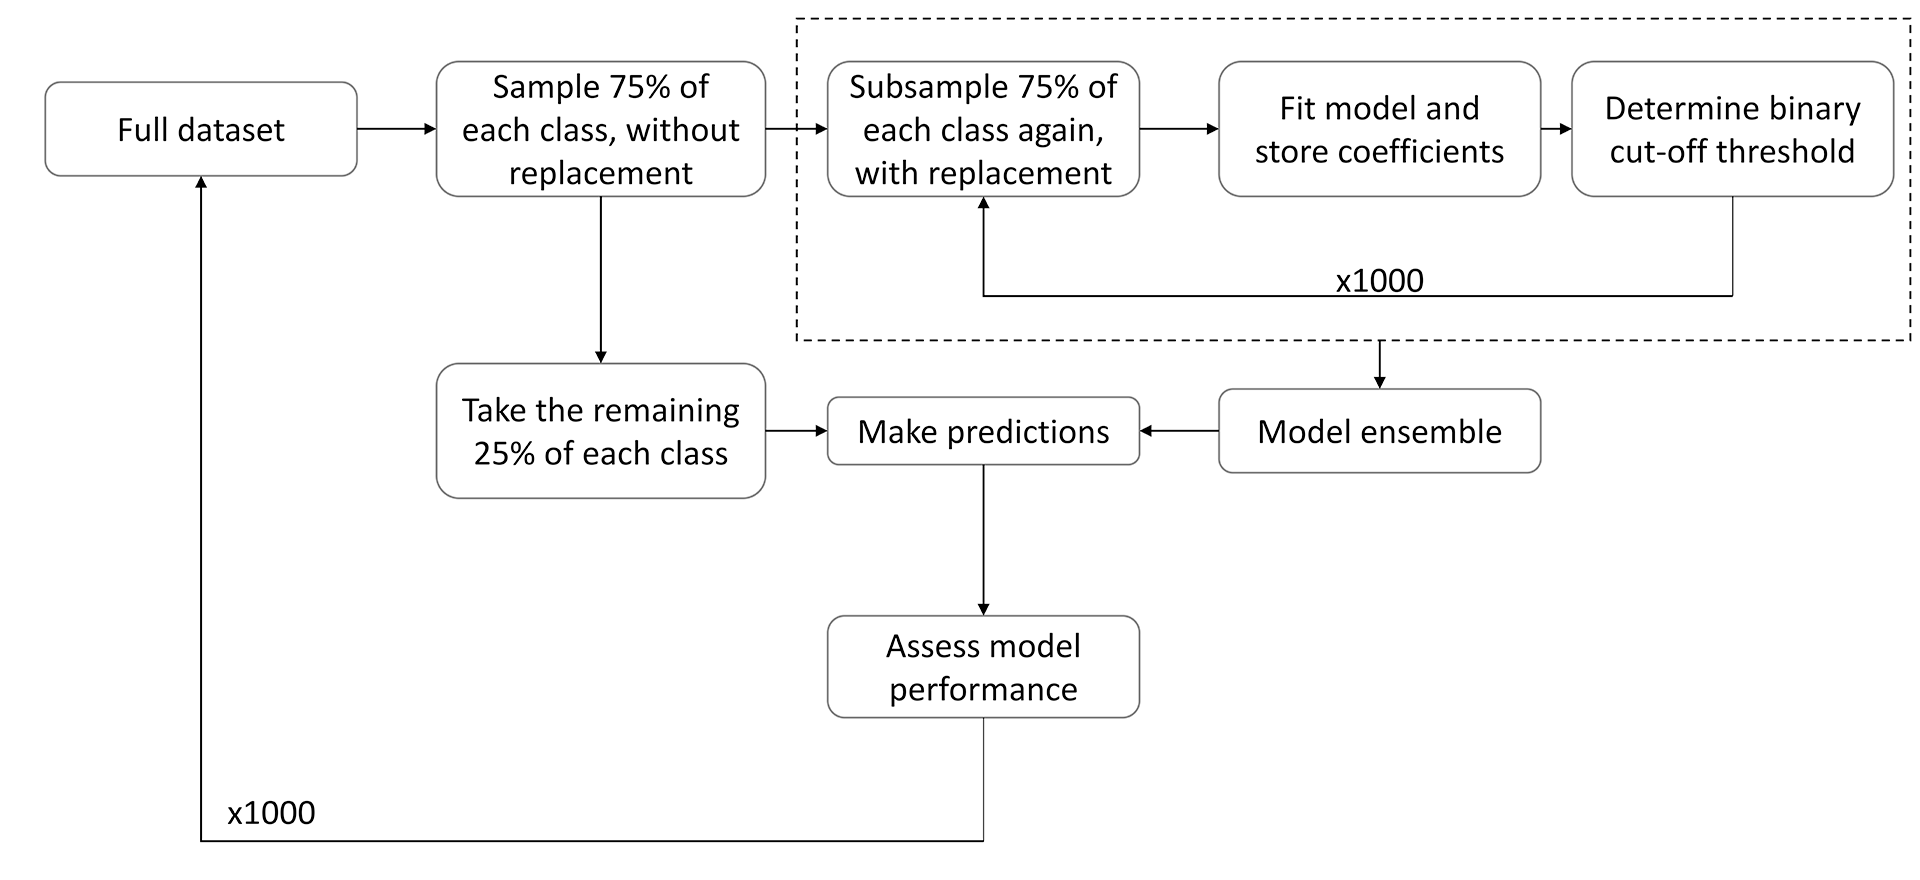
\includegraphics[width=\textwidth]{bootstrap_aggregation}
    \caption{Flowchart detailing the iterative bootstrap aggregation modelling process. The dotted box represents the `inner loop' for determining model coefficients. The remainder of the flowchart is the `outer loop' for assessing model performance. This process was carried out separately on the `Original' and `Additional' datasets.}
    \label{fig:bagging-flowchart}
\end{figure}

Modelling was carried out using a bootstrap aggregation process \cite{Hothorn2003}, in which an ensemble of models are trained on sub-samples of the full dataset. These are then used to generate predictions via a `majority votes' system, where each model in the ensemble predicts the outcome for each individual, and the most-predicted class is taken as the final prediction.
% All done twice - once on ace referral data, once plus additional features
The full modelling process is detailed below, and schematically in \Cref{fig:bagging-flowchart}. This process was carried out twice; once for the `Original' dataset and lasso-determined model structure, and once for the `Additional' dataset and lasso-determined model structure.

% Rationale
In summary, the process consists of an `inner' and `outer' loop.
% Inner loop to prevent overfitting and produce robust coefficients
The inner loop is iterated upon to prevent model overfitting, given the small absolute number of positive cases (i.e, hospitalisations), and to produce robust estimates for each variable in the model.
% Outer loop to generate distributions of model performance measures
The outer loop is iterated upon in order to generate distributions of each metric of model predictive performance, to allow us to fully assess the extent to which these metrics differ between the two models.

\subsubsection{Outer loop: Assessing model performance}
\label{sec:additional-model-performance}

The outer loop begins by splitting the full dataset into a training set comprising 75\% of positive cases and 75\% of negative cases, and a validation set comprising the remaining 25\%. Using the training set, an ensemble of logistic regression models are created (see \Cref{sec:additional-inner-loop}), each with the structure determined by the lasso process (see \Cref{sec:additional-model-structure}), but with their own values for each coefficient and prediction threshold.

Hospitalisation is then predicted using each model in the ensemble for each individual patient in the validation set. Each model uses its own prediction threshold and `votes' for the patient to be predicted as requiring hospitalisation or not. The majority case is then taken as that patient's predicted outcome.

% Details on metrics: https://topepo.github.io/caret/measuring-performance.html
With these predicted outcomes, 12 metrics of predictive performance were then calculated. These metrics are calculated from four rates: False positive ($F^+$), true positive ($T^+$), false negative ($F^-$), and true negative ($T^-$), shown in \Cref{tab:positivity-rates}.

\begin{figure}[H]
    \renewcommand\arraystretch{1.2}
    \centering
    \begin{tabular}{l|ll}
	& \textbf{Observed} &\\
	\textbf{Predicted} & Hospitalised & Discharged\\
	\hline
	Hospitalised & \quad\quad$T^+$ & \quad\quad$F^+$\\
	Discharged & \quad\quad$F^-$ & \quad\quad$T^-$\\
    \end{tabular}
    \caption[Schematic depiction of false and true positives and negatives]{Schematic depiction of false and true positives and negatives. $T^+$ = true positive, $F^+$ = false positive, $T^-$ = true negative, $F^-$ = false negative}
    \label{tab:positivity-rates}
\end{figure}

\textbf{Recall} (sometimes termed `sensitivity') and \textbf{precision} are defined in \Cref{subsec:evaluating-models}, and both measure the ability of the model to predict positive cases correctly. Recall is calculated as

\begin{equation}
Recall = \frac{T^+}{T^+ + F^-}
\end{equation}

and precision is calculated as

\begin{equation}
Precision = \frac{T^+}{T^+ + F^+}
\end{equation}

% Specificity, true negative rate
Similarly, \textbf{specificity} is the proportion of negative predictions which are true negatives, calculated as

\begin{equation}
Specificity = \frac{T^-}{T^- + F^+}
\end{equation}

% Accuracy
\textbf{Accuracy} is calculated as the number of correct predictions ($T^+$ + $T^-$) divided by the total number of predictions made. In cases such as the ACE data, where positive cases are much rarer than negative cases, accuracy can be as high as the prevalence of the largest category (in this case, 82.6\%) by a model that simply constantly guesses the largest category.
% Balanced accuracy: Average correct prediction proportion in each class
This can be remedied by\textbf{ balanced accuracy}, which gives the average proportion of correct predictions in both classes, calculated as
\begin{equation}
Balanced\;accuracy = \frac{Recall + Specificity}{2}\label{eq:balanced-accuracy}
\end{equation}

% AUC
Similar to balanced accuracy is \textbf{AUC}, which measures between 0.5 and 1 the ability of the model to discriminate between postive and negative cases (see \Cref{subsec:evaluating-models}). 
% Detection prevalence - Predicted positives out of total predictions
\textbf{Prevalence} gives the number of \textit{predicted} positives as a proportion of total predictions, calculated as
\begin{equation}
Prevalence = \frac{T^+ + F^+}
{T^+ + F^+ + T^- + F^-}
\end{equation}

% Detection rate
Closely related to detection prevalence is \textbf{detection rate}, the number of \textit{true} positives as a proportion of total predictions.



% NPV - Proportion of predicted negatives which are true negatives
Two metrics can quantify the ability of the model to predict negative cases and positive cases respectively. \textbf{Negative predictive value} (NPV) is the proportion of predicted negatives which are true negatives, calculated as

\begin{equation}
NPV = \frac{Recall \times (1-Prevalence)}
{((1-Recall) \times Prevalence) + (Specificity \times (1-Prevalence)}
\end{equation}

% PPV - Proportion of predicted positives which are true positives (= precision)
Similarly, \textbf{Positive predictive value} (PPV) is the proportion of predicted positives which are true positives, calculated as

\begin{equation}
PPV = \frac{Recall \times Prevalence}
{(Recall \times Prevalence) + ((1-Specificity) \times (1-Prevalence)}
\end{equation}

Note that PPV should also be equal to recall, though its derivation is different. Finally, we calculated two combined metrics of model performance:
% F1 - Trade-off between precision and sensitivity, explained and defined in \Cref{subsec:evaluating-models} and \Cref{eq:F1}
\textbf{F1} represents the model's trade-off between precision and recall, explained in \Cref{subsec:evaluating-models} and defined in \Cref{eq:F1}. \textbf{Cohen's kappa} ($\kappa$) measures the increase in performance of the model being assessed, compared to a theoretical model that guesses randomly, but following the frequencies of each outcome \cite{Landis1977}. For a binary outcome, it is calculated as

\begin{equation}
\kappa = \frac{2 \times ((T^+ \times T^-) - (F^- \times F^+))}
{((T^+ + F^+) \times (F^+ +  T^-)) + ((T^+ + F^-) \times (F^- +  T^-))}
\end{equation}

and yields a value usually between 0 and 1, where greater values indicate increasing performance (though negative values are possible).

% Outer loop repeated 1,000 times
The outer loop is repeated 1,000 times to allow a distribution of values to be built for each model performance metric. This allows the assessment of differences in these metrics between the `Original' and `Additional' models.

 	
\subsubsection{Inner loop: Determining model coefficients}
\label{sec:additional-inner-loop}

% Inner loop
The inner loop begins by receiving the training set from the outer loop (see \Cref{sec:additional-model-performance}). The training set is then sub-sampled to 75\% of its full size \textit{with replacement}, maintaining proportions of positive to negative cases. Using this sub-sampled dataset, a logistic regression model is fitted with the structure determined in \Cref{sec:additional-model-structure}, yielding an estimate for each model coefficient.

To determine the optimal threshold of the model for converting the log-odds of hospitalisation generated by the model into a binary predicted outcome, we profile a range of potential thresholds. At each candidate threshold value, the model is used to predict the log-odds of hospitalisation for the same individuals used to train the model. These predictions are then binarised using the candidate threshold, and balanced accuracy is determined (see \Cref{eq:balanced-accuracy}). The prediction threshold giving the greatest balanced accuracy is then recorded along with the model coefficient estimates.

This loop is carried out 1,000 times per training set, in order to produce a model ensemble which is robust to the specifics of the small number of positive cases upon which each individual model is trained.

% Table of N, in each category + coefHDI
\begin{table}[h]
\centering
\caption[Prevalence and model coefficients for retained variables.]{Prevalence and model coefficients for retained variables for the `Original' and `Additional' models. For binary variables, we present the number of patients for which the variable is true, and the percentage of patients in that group (discharged or hospitalised) which that represents. For continuous variables, we present the median value with lower and upper quartiles. Model coefficients are the result of the bootstrap aggregation process, and are presented as medians with lower and upper highest density intervals (HDI)}
\begin{tabular}{P{5cm}P{2.5cm}P{2.5cm}l}
  \hline
Variable (`Original' model) & Discharged from ACE & Admitted to Hospital & Coefficient \\ 
  \hline
Intercept & --- & --- & -2.61 [-2.96, -2.27] \\ 
  Abnormal respiratory rate & 78 (21.2\%) & 23 (29.5\%) & 0.55 [0.2, 0.94] \\ 
  Food allergy & 38 (10.3\%) & 11 (14.1\%) & 0.37 [-0.16, 0.79] \\ 
  Heart rate & 120 [109, 130] & 120 [117, 132] & 0.19 [0.03, 0.41] \\ 
  Moderate illness severity & 44 (12\%) & 15 (19.2\%) & 0.35 [-0.08, 0.8] \\ 
  Mentions asthma & 53 (14.4\%) & 20 (25.6\%) & 0.92 [0.56, 1.38] \\ 
  Mentions salbutamol & 59 (16\%) & 19 (24.4\%) & 0.36 [-0.01, 0.74] \\ 
  Oxygen saturation & 97 [96, 98] & 96 [95, 97] & -0.32 [-0.49, -0.15] \\ 
  Referral from GP & 199 (54.1\%) & 55 (70.5\%) & 0.72 [0.36, 1.09] \\ 
  \hline
Variable (`Additional' model) & Discharged from ACE & Admitted to Hospital & Coefficient \\ 
  \hline
  Intercept & --- & ---& -2.99 [-3.36, -2.61] \\
  Any eczema diagnosis & 160 (43.7\%) & 49 (62.8\%) & 0.77 [0.41, 1.11] \\ 
  High local NO2 & 58 (16.1\%) & 22 (28.2\%) & 0.75 [0.34, 1.1] \\ 
  Mentions asthma & 53 (14.4\%) & 20 (25.6\%) & 0.52 [0.07, 0.94] \\ 
  Oxygen saturation & 97 [96, 98] & 96 [95, 97] & -0.42 [-0.57, -0.24] \\ 
  Any pneumonia diagnosis & 40 (10.9\%) & 19 (24.4\%) & 1.05 [0.60, 1.46] \\ 
  Referral from GP & 199 (54.1\%) & 55 (70.5\%) & 0.60 [0.27, 1.00] \\ 
  Slow bronchodilators in last year & 78 (21.3\%) & 29 (37.2\%) & 0.37 [0.04, 0.77] \\ 
   \hline
\end{tabular}
\end{table}

\section{Results}

\subsection{Retained variables}

Our lasso logistic regression retained the following variables from the `Original' dataset: Abnormal respiratory rate (i.e., not in the `normal' APLS category), presence of food allergies, increasing heart rate, illness severity classified as `moderate' upon examination, mention of `asthma' in medical history, mention of `salbutamol' in the examination notes, decreasing oxygen saturation, and if the referral was made by the patient's GP. Further details on these variables can be found in the upper portion of \Cref{tab:additional-retained-variables}, and a graphical representation of the resulting model coefficients can be seen in the upper panel  \Cref{fig:additional-coefficients}.

In the `Additional' dataset, the mention of asthma, oxygen saturation and referral from GP were retained, as in the `Original' dataset. Further to this, lasso logistic regression also retained the following new variables: Any diagnosis of eczema, any diagnosis of pneumonia, prescription of slow bronchodilators in the year prior to ACE acceptance, and the patient's home being in an area of high NO$_2$ air pollution (>18.5 $\mu$g$\cdot$m$^3$). Further details on these variables can be found in the lower portion of \Cref{tab:additional-retained-variables}, and a graphical representation of the resulting model coefficients can be seen in the lower panel  \Cref{fig:additional-coefficients}. No variables from the demographic, prescriptions, distance or socio-economic deprivation groups were retained by the model.



% Also as 2 panel figure of posteriors
\begin{figure}[h]
    \centering
    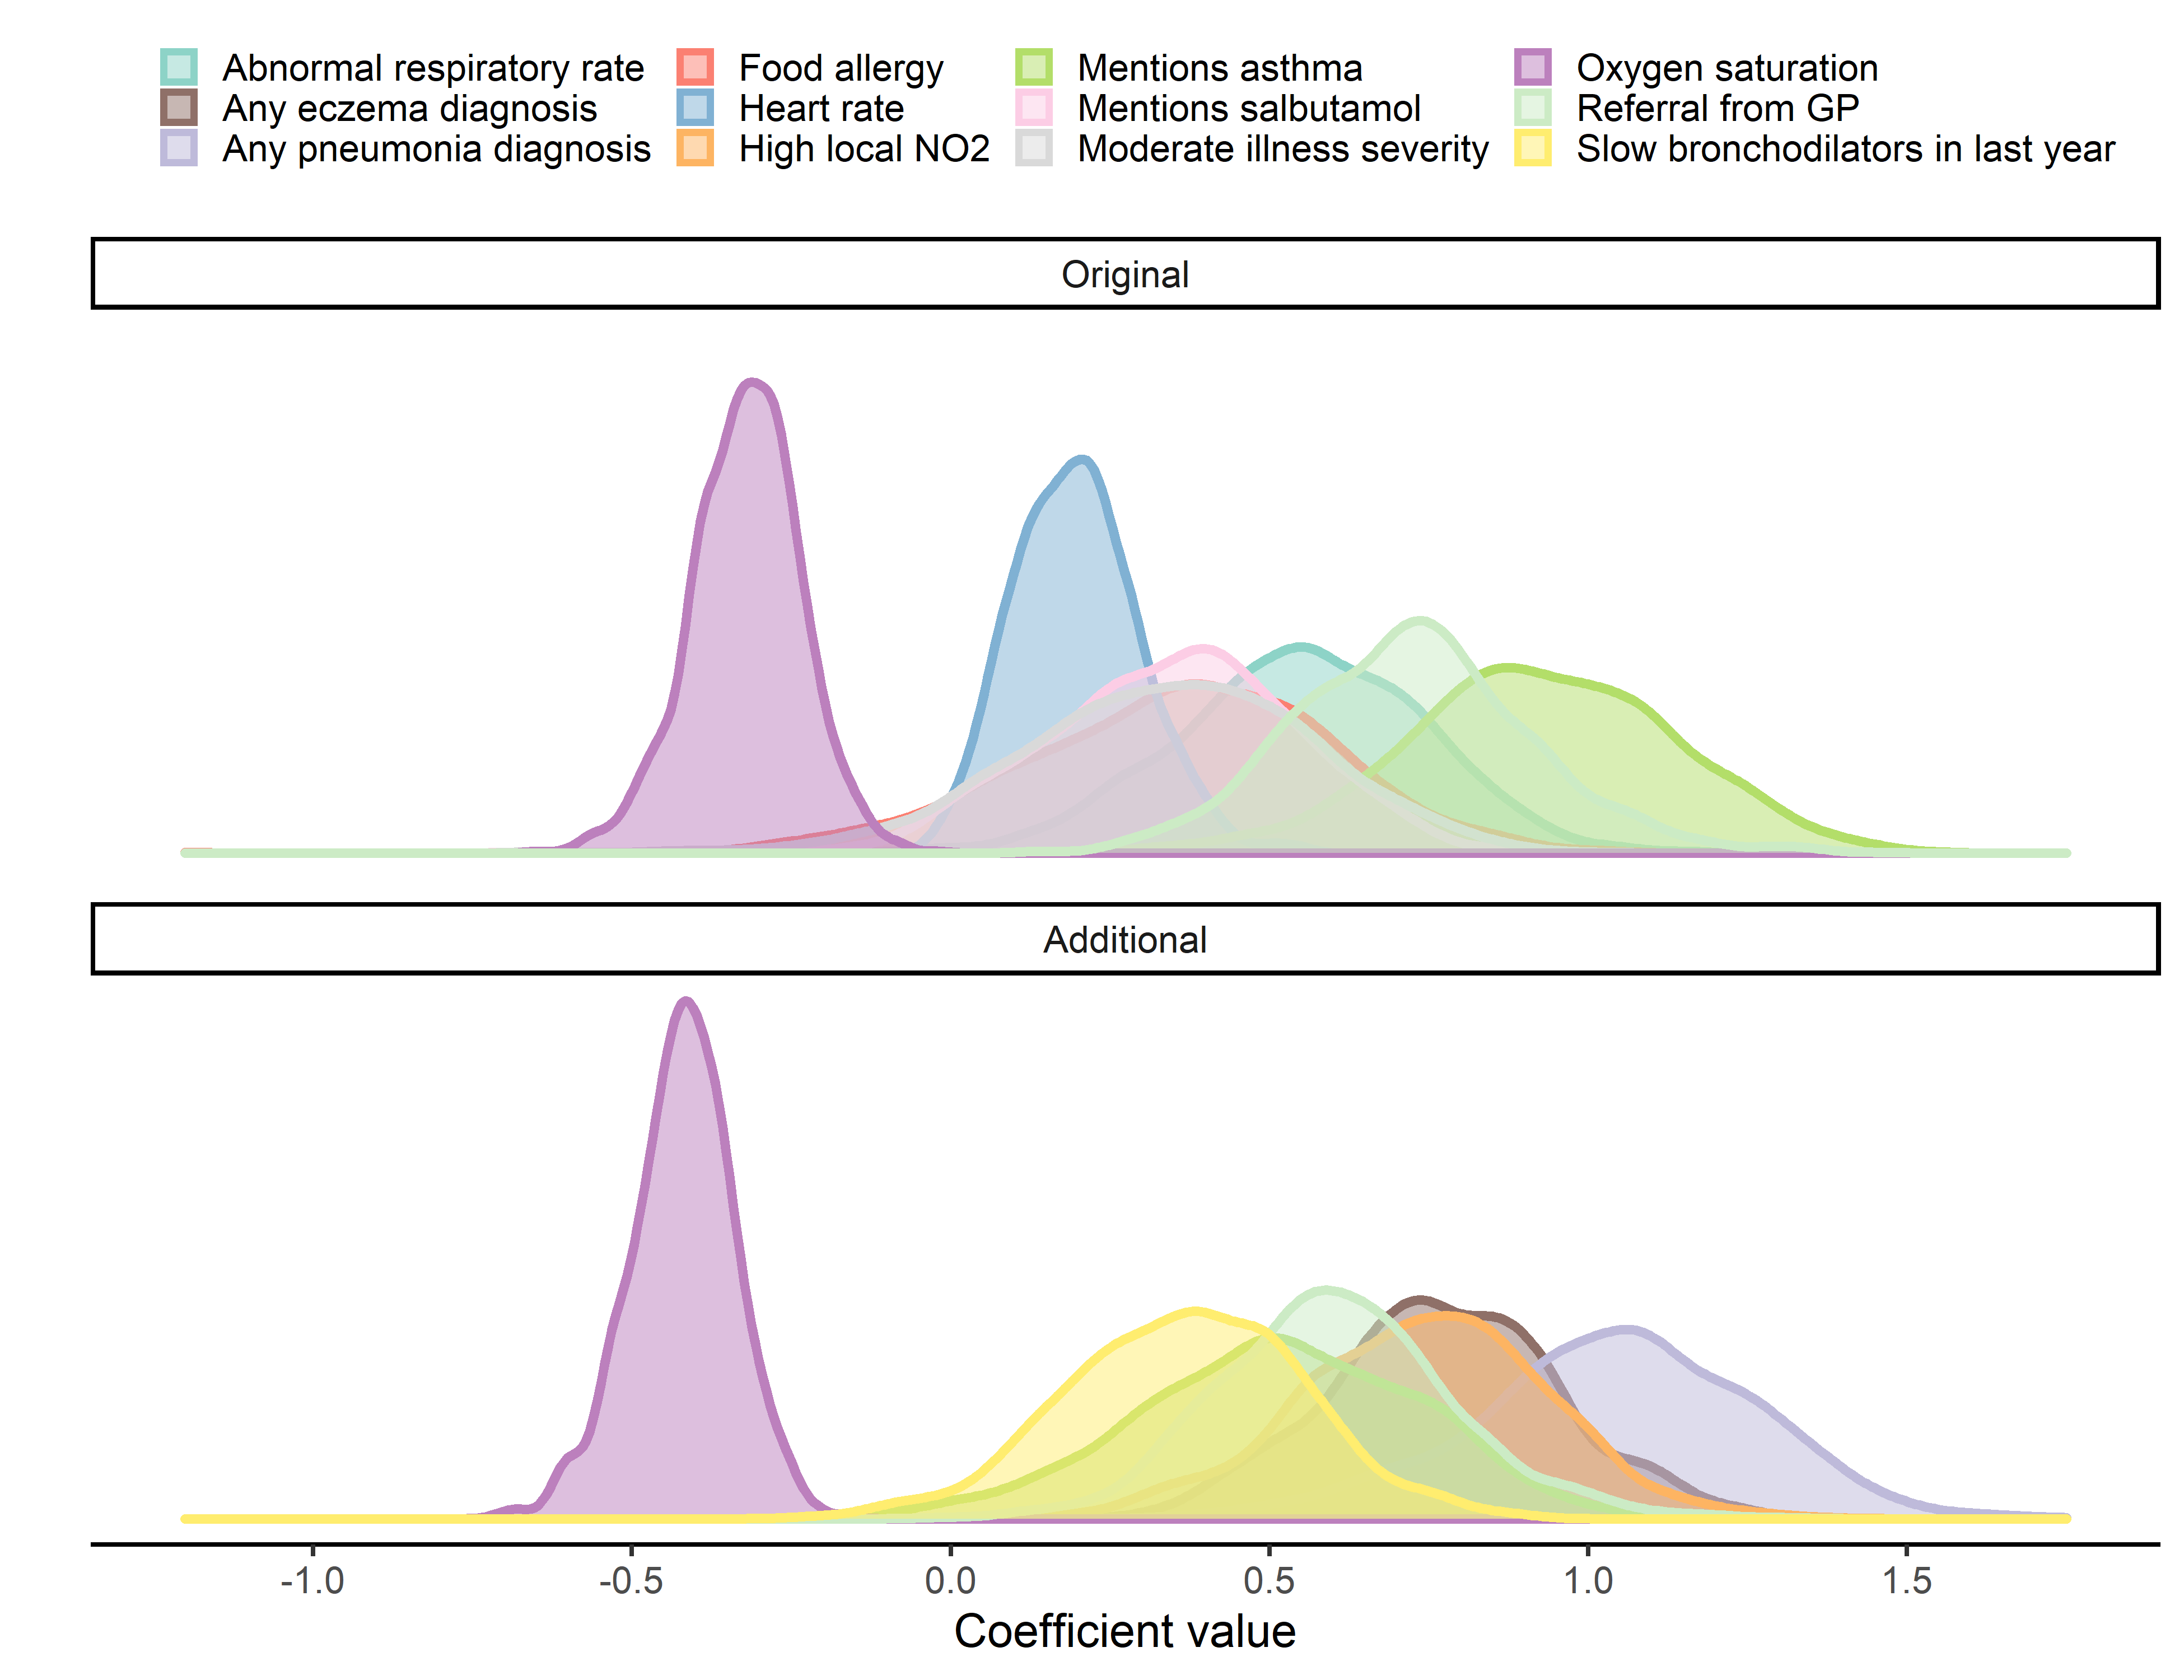
\includegraphics[width=\textwidth]{additional_coefs}
    \caption[Kernal density plots of estimated coefficients for `original' and `additional' models]{Kernal density plots of estimated coefficients for `original' and `additional' models. Features shared between the two models are coloured consistently between the two plots.}
    \label{fig:additional-coefficients}
\end{figure}

\subsection{Model performance}

% Table 
\begin{table}[h]
\centering
\caption[Comparison of model performance metrics]{Comparison of model performance metrics (see \Cref{sec:additional-model-performance}) between `Original' and `Additional' models. Metrics are presented as median values with upper and lower quartiles. `Ratio' is the ratio of the median performance metric value of the `Additional' model to the median performance metric value of the `Original' model.}
\begin{tabular}{P{4.5cm}P{3cm}P{3.15cm}P{1.5cm}}
  \hline
Metric & `Original' model & `Additional' model & Ratio\\
  \hline
  Accuracy & 0.66 [0.63, 0.69] & 0.69 [0.66, 0.72] & 1.05 \\ 
  AUC & 0.60 [0.56, 0.64] & 0.64 [0.60, 0.68] & 1.07 \\ 
  Balanced Accuracy & 0.60 [0.56, 0.64] & 0.64 [0.60, 0.68] & 1.07 \\ 
  Prevalence & 0.34 [0.31, 0.38] & 0.33 [0.30, 0.37] & 0.97 \\ 
  Detection Rate & 0.09 [0.08, 0.11] & 0.10 [0.09, 0.12] & 1.11 \\ 
  F1 & 0.34 [0.30, 0.39] & 0.39 [0.35, 0.44] & 1.15 \\ 
  Kappa & 0.14 [0.09, 0.20] & 0.21 [0.15, 0.26] & 1.50 \\ 
  Negative Predictive Value & 0.87 [0.85, 0.88] & 0.88 [0.86, 0.90] & 1.01 \\ 
  Positive Predictive Value & 0.26 [0.23, 0.29] & 0.30 [0.27, 0.33] & 1.15 \\ 
  Precision & 0.26 [0.23, 0.29] & 0.3 [0.27, 0.33] & 1.15 \\ 
  Recall & 0.50 [0.45, 0.60] & 0.55 [0.50, 0.65] & 1.10 \\ 
  Specificity & 0.70 [0.65, 0.73] & 0.72 [0.68, 0.75] & 1.03 \\ 
   \hline
\end{tabular}
\label{tab:additional-retained-variables}
\end{table}

% Figure
\begin{figure}[h]
    \centering
    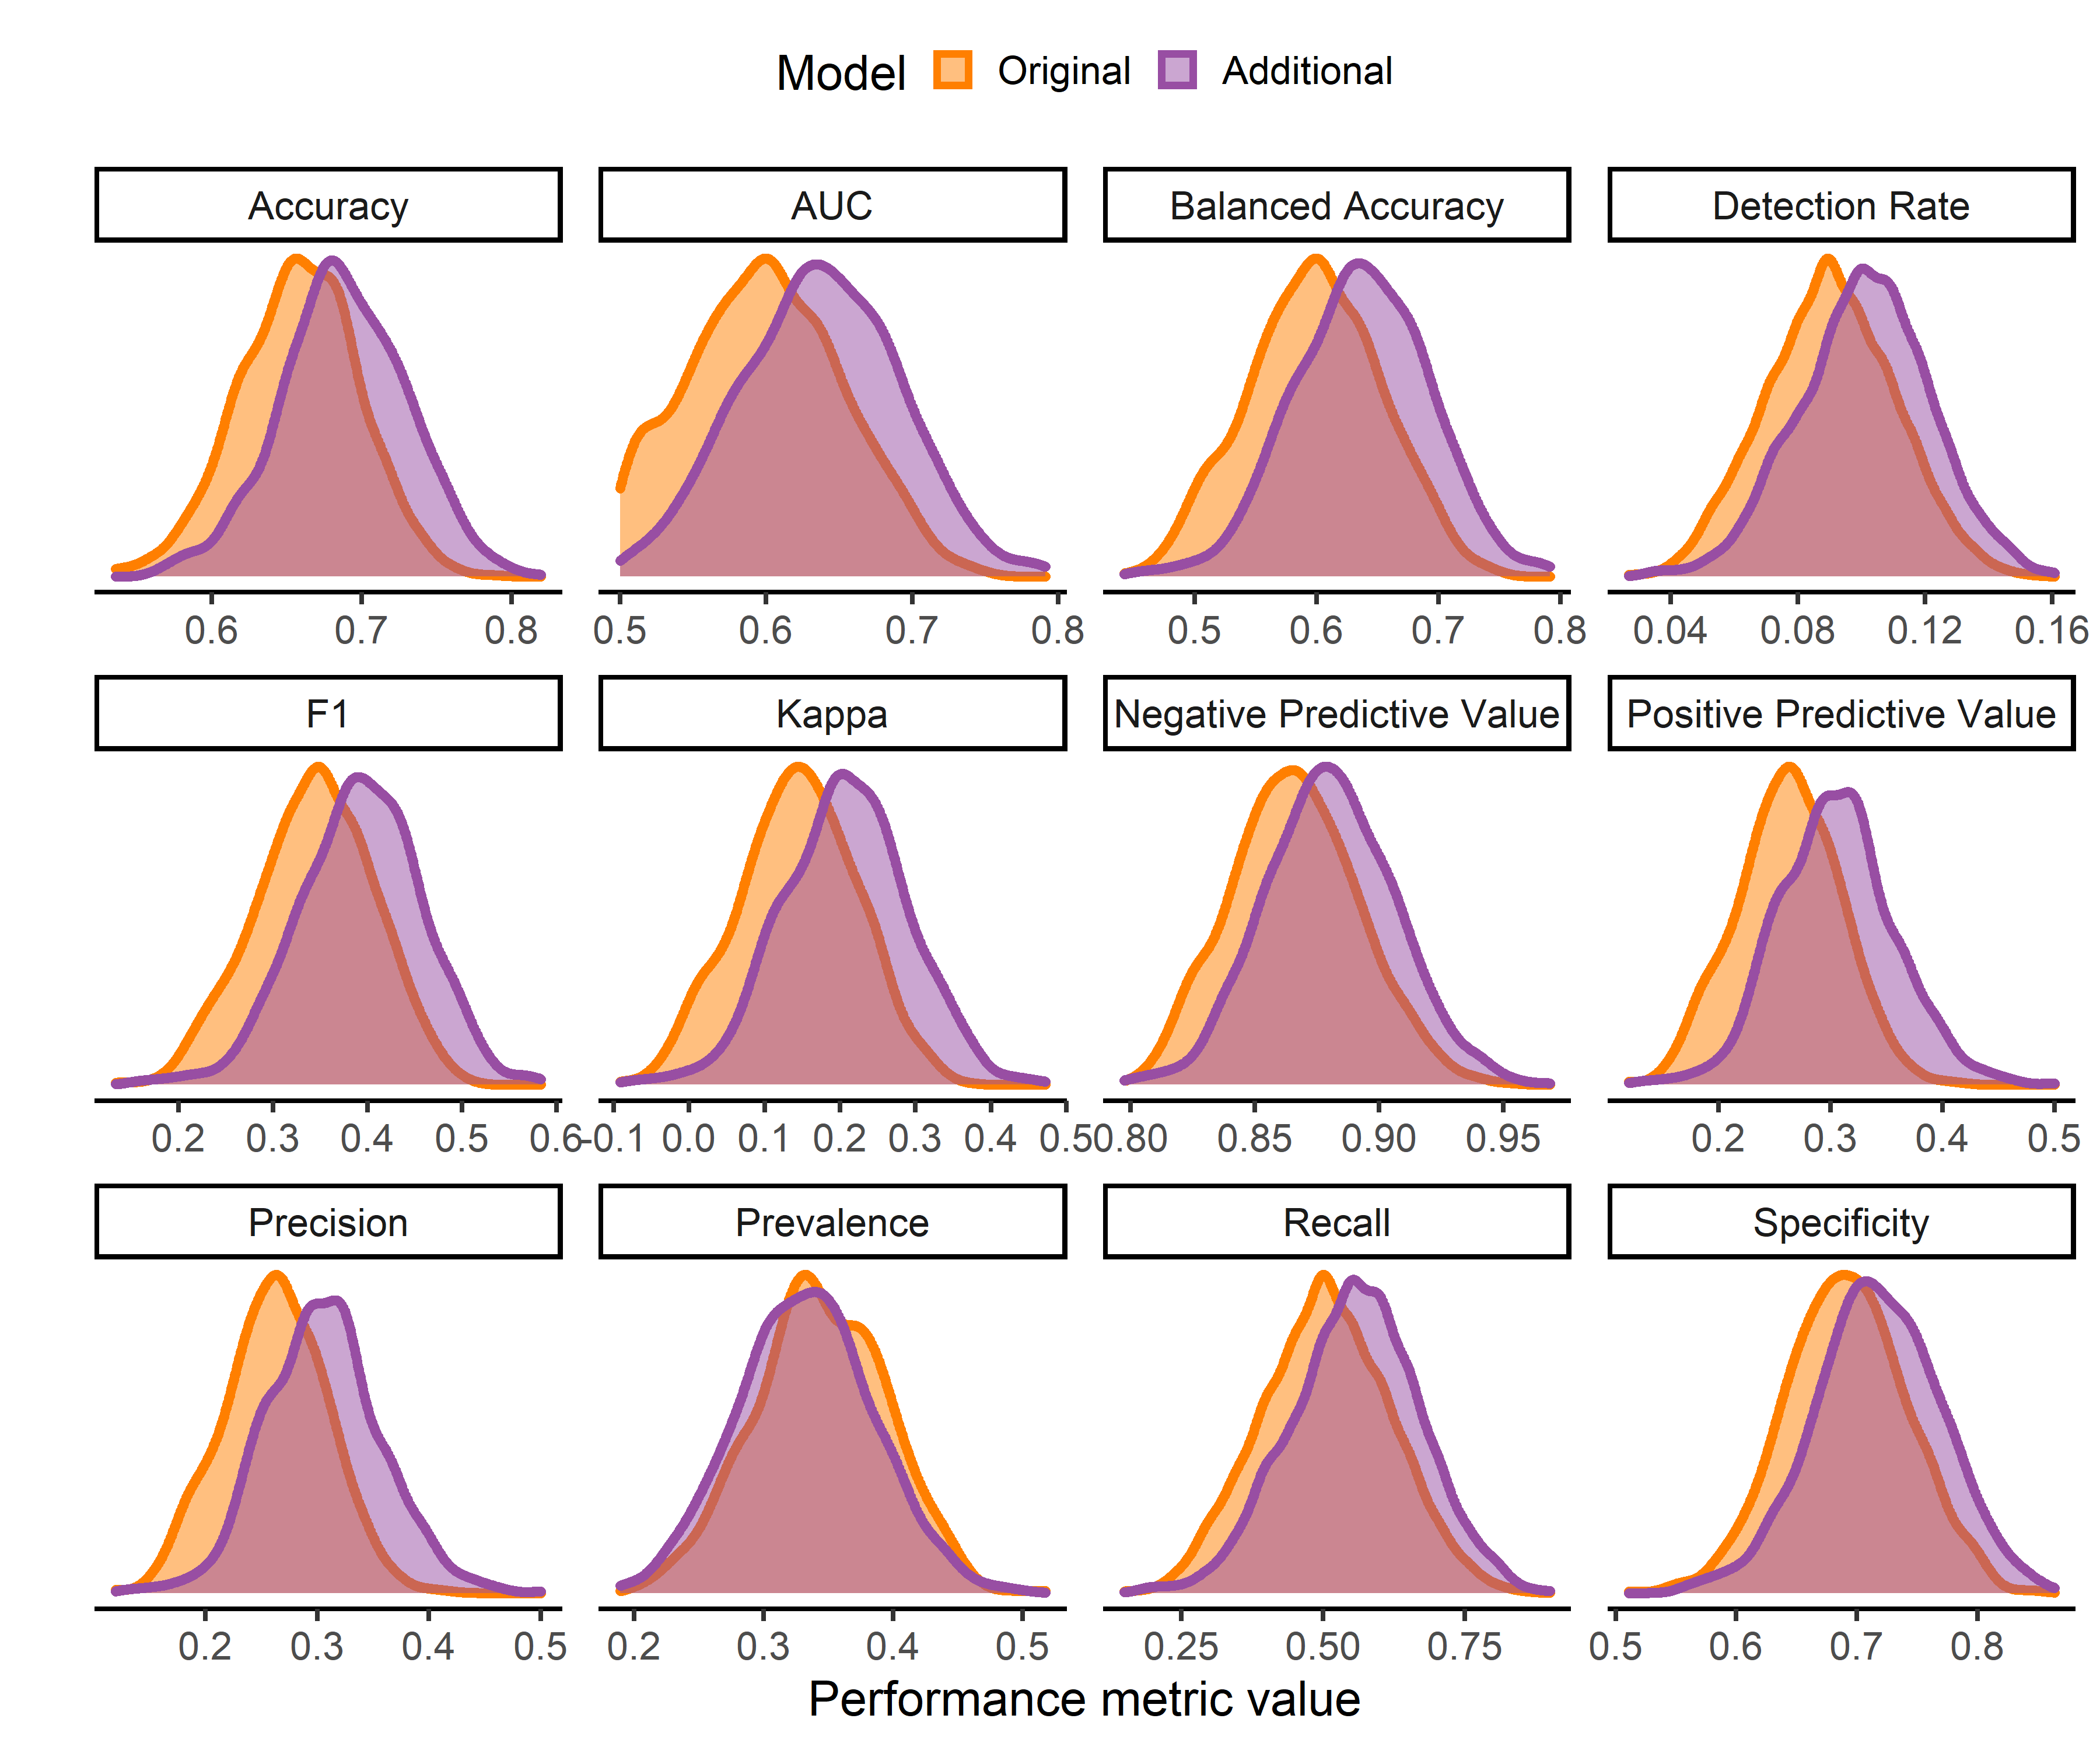
\includegraphics[width=\textwidth]{additional_performance}
    \caption[Kernal density plots comparing model performance metrics]{Kernal density plots comparing model performance metrics (see \Cref{sec:additional-model-performance}) between `original' and `additional' models. }
    \label{fig:additional-performance}
\end{figure}

% All better in `additional', 
In all but one measure of model performance, the `Additional' model showed superior performance to the original model. \Cref{tab:additional-retained-variables} shows these differences in detail, and \Cref{fig:additional-performance} depicts these differences graphically. Prevalence, the number of predicted hospitalisations as a proportion of the total number of predictions made, did not differ between the two models, and nor would we expect it to. As the training data contained fixed and unbalanced proportions of hospitalisations to non-hospitalisations, it would be expected that prevalence be equal in the two models.

% Increase performance seems to come more from an increase in ability to detect positive cases
Our results also show that this increase in performance comes from the increased ability of the `Additional' model to predict hospitalisations, as opposed to increased ability to detect patients who will not be hospitalised. We see, for example, a 1.15-fold increase in the positive predictive value (from 0.26 [0.23, 0.29] in the `Original' model to 0.30 [0.27, 0.33] in the `Additional' model), but only a 1.01-fold increase in the negative predictive value (from 0.87 [0.85, 0.88] in the `Original' model to 0.88 [0.86, 0.90] in the `Additional' model). This can also be seen in the 1.10-fold increase in recall (from  0.50 [0.45, 0.60] in the `Original' model to 0.55 [0.50, 0.65] in the `Additional' model), with again only a 1.03-fold increase in specificity (from  0.70 [0.65, 0.73] in the `Original' model to 0.72 [0.68, 0.75] in the `Additional' model).

% but not by much
Whilst the `Additional' model does out-perform the `Original' model, we must still consider its objective performance as a classifier. A median Cohen's kappa of 0.21 [0.15, 0.26] denotes only `fair' performance \cite{Landis1977}, and similarly, a median AUC of 0.64 [0.60, 0.68] is generally considered to denote `moderate' predictive performance.

\section{Discussion}

As with the results in presented in earlier chapters, our results as presented here do not allow the development of a functional model to predict hospitalisation for patients referred to the ACE service. Whilst the models containing additional variables do perform better than those trained on just the data from the ACE referral form, their objective performance is still, at best, mediocre. The insights from these models, however, do allow us to make some recommendations and considerations, both for improvements to the ACE admissions pathway, and for future study in this area.

\subsection{Considerations for ACE admissions}

% Eczema, pneumonia, bronchodilator use, referral source
Of the many additional variables that correlated with increased hospitalisation risk, only a small number were retained in the final model. Whilst this does not mean necessarily that non-retained variables were spurious correlations, it \textit{does} imply the importance of those that were retained. In terms of medical history, past diagnoses of pneumonia, eczema, and food allergies were retained in the models, along with prescription of long-acting bronchodilators. This information would or could likely be known either to ACE admissions staff, or to parents of patients, at the point of referral. Therefore, we recommend that investigation of these co-morbidities and medical histories be investigated further for their association with ACE referral and subsequent hospitalisation, and that the ACE team consider overtly asking about eczema, pneumonia and bronchodilator prescription when assessing a patient for acceptance onto the service.

% GP
Similarly, in both models, patients referred to ACE from their GP were at greater risk of hospitalisation. Whilst it is unclear from the data what the causal pathway is here, this finding suggests that the origin of a patient's referral should also be considered when assessing prospective ACE patients.

\subsection{Considerations for future study}

This analysis has highlighted a number of fruitful avenues for future research to investigate more thoroughly.
% Mentions asthma was preferred to a formal diagnosis
First, the mention of `asthma' in the examination notes was not only retained it both models, but was also retained in the `Additional' model despite the presence of variables containing actual information on asthma diagnosis. This suggests that the mention of asthma in the notes is more important than whether or not the patient actually has asthma. 
% Sentiment analysis for free text stuff
This could be, for example, because notes might only tend to mention a patient's asthma if it is relevant, problematic or not under control. Additional analysis of the examination notes such as a sentiment analysis may be able to indicate where mentions of asthma are linked with language indicating that the patient's asthma is potentially problematic, thus improving its predictive power.

% NO2 and correlated variables
Second, the `Additional' model identified patients from areas of high background air pollution (NO$_2$) as being at higher risk of hospitalisation. Whilst a link between air pollution and hospitalisation for asthma-like respiratory conditions makes logical sense, our results to not permit us to interpret this as a causal relationship, for several reasons. First, our air quality data are estimated, rather than measured. Whilst measured data are available, there are few recording stations in the Bradford area, so estimated local concentrations were determined to be more accurate than concentrations measured further away, as air pollution levels tend to be geographically heterogeneous. Second, our analysis was restricted to the LSOA levels. This comes with a number of assumptions, including the assumption that air pollution is heterogeneous across a given LSOA, and the assumption that the pollution levels in a given LSOA are in fact the levels that children are exposed to. Further study could therefore account for how much children move between neighbouring LSOAs, especially, for example, for school. Finally, the `High NO$_2$' feature could simply be capturing any number of other geospatial variables, such as socio-economic deprivation, local access metrics, or the quality of local healthcare services. Subsequent work should therefore focus on demonstrating a direct causal link between exposure to increased air pollution, and a greater likelihood of being hospitalised with asthma or related respiratory conditions.

% Other variables of interest may give useful predicitve value given more cases
Finally, our work identified a number of variables across prescriptions, healthcare visits, accessibility measures and socio-economic deprivation which correlated with increased hospitalisation risk in a univariate model, but were not retained by final models. One major reason for this is likely due to the number of variables being retained by the model being highly constrained by the low number of positive cases, even with mitigation strategies against overfitting. Future work in this area with a greater number of cases could more thoroughly investigate relationships between the additional `variables of interest' highlighted here, and the risk of hospitalisation.